
\documentclass[11pt]{article}

\usepackage{amsmath}
\usepackage{amsfonts}
\usepackage{mathtools}
\usepackage[ruled,vlined,noend]{algorithm2e}
\usepackage{algpseudocode}
\usepackage{fancyvrb}
\usepackage{booktabs}

\newtheorem{example}{Example}[section]
\newtheorem{definition}{Definition}[section]


\begin{document}
    \title{Detection of markers for discrete phenotypes}
    \author{Hannes Klarner$^1$ \and Elisa Tonello$^1$ \and Elisa Tonello$^1$ \and Laura Cifuentes$^1$ \and Florence Janody$^2$ \and Claudine Chaouiya$^3$ \and Heike Siebert$^1$}
    \date{%
        $^1$Freie Universität Berlin, Berlin, Germany\\%
        $^2$Instituto de Patologia e Imunologia Molecular, Porto, Portugal\\%
        $^3$Institute of Mathematics of Marseille, Marseille, France\\[2ex]%
        November 2021
    }
    \maketitle

    \begin{abstract}
        \textbf{Motivation:}
        Capturing the molecular diversity of living cells is not straightforward.
        One approach is to measure molecular markers that serve as indicators of specific biological conditions or phenotypes.
        This is particularly relevant in modern medicine to provide precise diagnostics and pinpoint the best treatment for each patient.
        The challenge is to select a minimal set of markers whose activity patterns are in correspondence with the phenotypes of interest.

        \textbf{Results:}
        This article approaches the marker detection problem in the context of discrete phenotypes which arise, for example, from Boolean models of cellular networks.
        Mathematically this poses a combinatorial optimization problem with many answers.
        We propose a solution to this optimization problem that is based on the modelling language answer set programming (ASP).
        A case study of a death cell receptor network illustrates the methodology.

        \textbf{Discussion and code:}
        For code, discussions and reporting errors visit \verb+https://github.com/hklarner/detection_of_markers_for_discrete_phenotypes+.

        \textbf{Contact:}
        hannes.klarner@fu-berlin.de
    \end{abstract}

    \section{Introduction}
    \subsection{Biological background}
    In 2001, the National Institutes of Health's Biomarkers Definitions Working Group defined a biomarker as "a characteristic that is objectively measured and evaluated as an indicator of normal biologic processes, pathogenic processes, or pharmacologic responses to a therapeutic intervention", see~\cite{biomarkers2001biomarkers}.
    Among biomarkers, molecular biomarkers can disclose changes in gene copy number, gene mutations, alterations of the levels of gene or protein expression or variations of the functional activity of a component.
    They have a wide array of uses in a variety of fields, including medicine, developmental biology, and basic scientific research.
    In particular, the use of biomarkers has increased greatly in precision medicine to diagnose pathogenic processes, to assess patient prognosis, to select the best treatment for each individual, as well as to evaluate risk of developing diseases.
    However, the clinical translation of novel molecular biomarkers predicting disease susceptibility, progression or treatment outcome remains poor, in particular for complex diseases, such as Alzheimer and related forms of dementia, cancer, diabetes and heart disease, with less than two approvals per year across all diseases among thousands of potential identified biomarkers.
    This lack of success can arise from experimental limitations of the biomarker discovery pipeline.
    In addition, because these diseases consist of various pathophysiological processes, resulting from multiple molecular and environmental factors, and exhibit variable disease course and response to therapy, a single biomarker rarely fulfills all necessary criteria for a comprehensive diagnostic or prognostic assessment, see~\cite{antoranz2017mechanism}.
    There is therefore an unmet need for multi-marker discovery using biomarkers reflecting different pathophysiologies that could be used in routine clinical practice, see~\cite{ball2010evaluation}.
    Analysis of data in terms of complex networks may help to identify these key biomarkers.
    This path requires a multidisciplinary approach, engaging researchers in numerous fields: biologists, informatics specialists, and mathematicians.

    \subsection{Mathematical background}
    In its essence the marker detection approach proposed in this article is one of combinatorial optimization.
    The input to this problem consists of a list of binary vectors whose coordinates designate the available molecular components, and whose values indicate the activity or abundance of the respective component.
    Each vector is an abstract representation of a state of the biological system.
    Usually these states will belong to the long-term behaviors of the system, the so-called attractors, but technically this is not a requirement.

    We are aware of two distinct settings to which our work is applicable.
    First, such binarized states are the output of discretization algorithms that are frequently a preliminary step to the analysis of continous gene expression data.
    For an example in the context of time series data, see~\cite{dimitrova2010discretization}.

    Second, they are the principal output of discrete models of molecular interaction networks.
    A prominent example of discrete models are Boolean interaction networks.
    These consist of Boolean variables that are governed by fixed update functions and some assumption about the number of variables that are permitted to change state simultaneously during a state transition.
    While reachability questions, the enumeration of all attractors and descriptions of the basins of attraction are currently limited to medium-sized models of about 50 components, see~\cite{klarner2018basins}, the detection of steady states is feasible for large networks of hundreds of components and more, see for example~\cite{aracena2021finding}.
    In the context of this paper we assume that the steady states capture the phenotypes under investigation.
    For a survey on Boolean networks in systems biology, see for example~\cite{wang2012boolean, schwab2020concepts}.

    The overall challenge we are facing is therefore to nominate multi-element markers that are 1) minimal and therefore low cost, and 2) respect the practical limitations of available marker candidates.
    The relationship between the solutions of a marker detection problem and its underlying Boolean network model, if there is one, is also of interest.

    \subsection{Summary}
    The article is organized in five sections.
    Sec.~\ref{sec:definitions-and-notation} introduces the notation for Boolean networks and basic set theory required in this text.
    It is followed by Sec.~\ref{sec:markers-and-phenotypes} which defines phenotypes and marker types for steady states and introduces the notions of consistency and marker component equivalence.
    The methods section, Sec.~\ref{sec:materials-and-methods}, gives details on our ASP encoding of the marker detection problem.
    A case study which illustrates the full methodology for a death cell receptor model published in~\cite{calzone2010mathematical} is presented in Sec.~\ref{sec:results}.
    The discussion and outlook are given in Sec.~\ref{sec:discussion}.

    \section{Definitions and notation}\label{sec:definitions-and-notation}
    A \emph{Boolean network} of $n$ components is an $n$-dimensional Boolean function $f=(f_1, \dots, f_n)$ with $f_i: \mathbb B^n \rightarrow \mathbb B$ where $\mathbb B = \{0,1\}$ are the Boolean values.
    A \emph{state} is a $n$-dimensional Boolean vector $x=(x_1, \dots, x_n)$.
    The synchronous update of a state $x$ is the image of $x$ under $f$, i.e., $f(x)=(f_1(x), \dots, f_n(x))$.
    A \emph{steady state} is a fixed point of $f$, that is, a state that satisfies $f(x) = x$.
    The \emph{interaction graph} is a directed graph $(V,A)$ where an arc $(i,j) \in A$ captures the dependence of $f_j$ on the variable $x_i$.

    \begin{example}[toy problem]
        The toy network consists of six components with two positive feedback loops $f_1=x_2, f_2=x_1, f_3=x_4, f_4=x_3$ and two read-out nodes whose update functions are $f_5=x_2 \wedge x_4, f_6=x_2 \vee (\neg x_2 \wedge \neg x_3)$.
        It has four steady states $S=\{000001, 110001, 001100, 111111\}$.
    \end{example}

    The \emph{power set} of a set $A$ is denoted by $\mathcal P(A) = \{B \mid B\subseteq A\}$.
    Given two families of subsets $\mathbf X, \mathbf Y \in \mathcal P (\mathcal P (X))$, we denote by $\otimes$ the set-product $\mathbf X \otimes \mathbf Y \coloneqq \{X \cup Y \mid X \in \mathbf X, Y \in \mathbf Y\}$.
    If $\mathbf Z = \mathbf X \otimes \mathbf Y$ we say that $\mathbf Y, \mathbf X$ are \emph{factors} of $\mathbf Z$.
    The set-product is often useful for giving concise descriptions of set families with many elements.

    An equivalence relation $\sim$ on a set $A$ induces a \emph{partition} of $A$ into $k$ \emph{blocks} $A_1, \dots, A_k$ with $A_i \subseteq A$ and $A_i\cap A_j=\emptyset$ for all $i,j$ and $A_1\cup \dots \cup A_k=A$.
    We call blocks of size one \emph{trivial blocks}.

    The number of elements of a set $A$ is denoted by $|A|$.

    \section{Markers and phenotypes}\label{sec:markers-and-phenotypes}

    The term phenotype refers to the classification of individual organisms by observable traits.
    The traits are determined, essentially, by the organism's genotype and the influence of environmental factors.
    More specifically, when studying mathematical models of biological systems, a phenotype usually refers to the expression pattern of specific components of interest under the assumption that the system has reached an attractor.

    In this text we focus on the steady states of a network and define the phenotypes by partitioning the steady states according to given phenotype components.
    Let $S$ be the steady states of a Boolean network and $P\subseteq V$ a set of \emph{phenotype components} with $|P|=k$.
    A \emph{phenotype} $p \in \mathbb B^k$ is the projection of a state $x \in S$ onto the phenotype components.
    We denote by $\pi_P: \mathbb B^n \rightarrow \mathbb B^k$ the \emph{projection} of $x$ onto $P$.
    For each phenotype $p$ we define the \emph{phenotype states} $\chi_p(S)$ by
    $\chi_p(S) \coloneqq \{x \in S \mid \pi_P(x) = p\}$.

    Analogously, we define \emph{marker components}, or \emph{markers} for short, as a subset $M \subseteq V$ and the \emph{marker-type} as a state of $M$.
    Note that, mathematically, markers and phenotypes are therefore objects of the same type.

    \begin{example}[toy problem]
        Suppose the phenotype components are $P=\{4,5\}$ and the marker components are $M=\{1,2\}$, then there are three phenotypes $\pi_P(S)=\{00, 10, 11\}$ and two marker-types $\pi_M(S)=\{00, 11\}$.
    \end{example}

    \subsection{Consistency between markers and phenotypes}
    In practice, we are given phenotype components and are asked to find marker components such that the phenotypes and the marker-types are consistent across all the steady states.
    That is, given only the marker-type of a steady state the phenotype must be uniquely deducible.

    \begin{definition}[consistency]
        The markers $M$ are \emph{consistent with} the phenotype components $P$ on $S$ iff $\forall x,x' \in S: \pi_M(x) = \pi_M(x') \implies \pi_P(x) = \pi_P(x')$.
    \end{definition}

    Note that this definition allows a 1-to-many relationship between the phenotypes and the marker-types on $S$.
    In practice this may introduce an unnecessary complexity in the experimental setup.
    If we are interested in 1-to-1 relationships we need to demand in addition that $P$ is consistent with $M$ in which case we say that $P$ and $M$ are \emph{equivalent}.

    Usually, to reduce the cost of adding markers or of reading marker values, we are furthermore interested in subset minimal markers $M$ and the \emph{exclusion constraint} which limits the marker candidate space to $M \subseteq U$ with $U = V \setminus P$.

    \begin{example}[toy problem]
        Suppose we are interested in subset minimal markers and the exclusion constraint.
        The markers $M=\{1,2\}$ are not consistent with $P=\{4,5\}$ because the steady states $x=000001, y=001100$ satisfy $\pi_P(x) = 00 \neq \pi_P(y)= 10$ but $\pi_M(x)=00 = \pi_M(y)$.
        The markers $M'=\{1,3\}$ are consistent with $P$ but $M'$ and $P$ are not equivalent because $|\pi_P(S)|=3$ and $|\pi_{M'}(S)|=4$.
        Finally, the markers $M''=\{3,6\}$ are equivalent to $P$.
        While $M''$ is the unique marker set that is equivalent to $P$, there is a family of three consistent marker sets, namely $\{\{1,3\}, \{2,3\}, \{3,6\}\}$.
    \end{example}

    \subsection{Marker component equivalence}
    Marker detection problems often have hundreds of solutions.
    We have noticed that this is partly due to an equivalence relation on $V$ that partitions $V$ into blocks of interchangeable components.
    In a sense, components within the same block carry the same information with regards to steady state identification.
    Intuitively, two components are equivalent if their activities are locked in a fixed relationship across all steady states under consideration.

    \begin{definition}[Steady state correlation]
        Two components $i,j \in V$ are \emph{correlated} across the steady states $S$ if either $\forall s,s'\in S: s_i = s_j$ or $\forall s,s'\in S: s_i \neq s_j$.
        We write $i \sim_S j$.
    \end{definition}

    The key observation is that correlated components are interchangeable in marker sets.
    That is, given $i,j \in V$ with $i \sim_S j$ and suppose that $i \in M$ for a marker set $M \subseteq V$.
    Then $M' \coloneqq (M \setminus \{i\}) \cup \{j\}$ is another valid marker set and of the same consistency type.

    Note that the steady state correlation is independent of the specification of phenotype components and therefore holds for all choices of $P$.
    In fact, the relation $\sim_S$ is an equivalence relation on $V$ and correlated components hence form blocks of a partition of $V$.

    \begin{example}[toy problem]
        The blocks of the steady state correlation are $\mathbf B=\{\{1,2\}, \{3,4\}, \{5\}, \{6\}\}$, two are trivial and two are non-trivial.
        Since $M=\{2,3\}$ is a marker set and $\{1,2\} \in \mathbf B$, it follows by the observation above that $M'=\{1,3\}$ is another valid marker set.
    \end{example}

    \section{Materials and methods}\label{sec:materials-and-methods}
    \subsection{Introduction to ASP}
    Answer set programming (ASP) is a particular form of logic programming.
    Mathematical problems are modelled in this language by stating rules over user-defined predicates.
    The answer sets of a program correspond to the solutions of the mathematical problem.
    ASP solvers like \emph{clasp}~\cite{gebser2007clasp} are capable of enumerating all subset minimal answer sets.

    ASP has been applied to problems in bioinformatics before, see for example the computation of minimal interventions in logical signaling networks \cite{kaminski_schaub_siegel_videla_2013}.
    The ASP modelling language is well-suited for combinatorial problems and the \emph{clasp} solver outperforms a brute force detection algorithm significantly.
    Encoding a mathematical problem in ASP and debugging can be tricky but small changes in the mathematical problem often correspond to small changes in the ASP program.
    In contrast, imperative programs often require large changes to adapt to variations of the mathematical problem.

    The following quick introduction to ASP is given in terms of the input language \emph{gringo}~\cite{gebser2012answer}.
    An \emph{atom} is a function symbol followed by terms which are either constants or variables.
    Examples of atoms are \verb+f(c,10)+ and \verb+g(X)+ where \verb+c+ and \verb+10+ are constants and upper-case letters, like \verb+X+, denote first-order variables.
    A \emph{rule} is a language construct that denotes an implication and consists of a \emph{head}, the implicant, and a \emph{body}, a conjunction of atoms followed by a full stop.
    The implication symbol is \verb+:-+ and means "if".
    An example is \verb+f(c) :- g(1), g(10)+ which makes \verb+f(c)+ true if both \verb+g(1)+ and \verb+g(10)+ are true.
    A rule without a body is called a \emph{fact} and its head is unconditionally considered true.
    Facts are a means of including data into the program.
    An \emph{answer set} consists of all atoms that are derivable by rules of the program.

    For our encoding of the marker detection problem we need two more \emph{gringo} language constructs.
    An \emph{integrity constraint} is a rule without a head.
    It serves as a solution filter that removes answer sets that satisfy the body.
    An example is \verb+:- f(a), g(10)+.
    A \emph{choice rule} is a construct for stating that any subset of set of atoms may be considered factual, i.e. as fact.
    It is often used to define the candidate space for combinatorial problems.
    An example is \verb+{f(1), f(5), f(12)}+.
    It states that any of the 8 subsets of the 3 atoms may be considered factual.
    Instead of enumeration, conditional statements using \verb+:+ are allowed and sometimes necessary.
    An example of a conditional choice rule is \verb+{f(I): g(I), not h(I)}+.
    Here, \verb+not h(I)+ is the \emph{classical negation} which evaluates to true for all values of $I$ for which \verb+h(I)+ can not be derived.
    The count of true atoms in a choice rule can be limited above and below by adding the integer values: \verb+3 {f(I): g(I), not h(I)} 10+.

    \subsection{Encoding of the marker detection problem}
    The first step is to encode the steady states.
    We use the predicate \verb+x(I,J,K)+ to encode the steady state data.
    Here, $0 \leq i < |S|$ is the identifier of a steady state, $j \in V$ is the index of a component and $k \in \mathbb B$ is the value of $j$ in the $i^{th}$ steady state.

    The following line numbers refer to Table~\ref{tab:toy_asp_encoding}.
    The predicate \verb+forbidden(J)+ states the indices $j \in V$ that are excluded from the marker detection problem.
    The phenotype components are declared by the predicate \verb+p(J)+ where $j \in V$.
    The marker component candidates are encoded by the predicate \verb+m(J)+ and defined via the choice rule in Line~\ref{line:markers}.
    Here, the underscores in the predicate \verb+x+ are place holders for which \emph{clasp} allows any value.

    Next we introduce the predicate \verb+different_phenotype(S1,S2)+ for steady states $s, s' \in S$ to be true if their phenotypes are different.
    Since the steady states are Boolean vectors we may simply enumerate the two cases under which $s, s'$ are of different phenotype, namely if there is a phenotype component for which the expression in the steady states differs.

    Note that we could instead introduce \verb+equal_phenotype(S1,S2)+, but it is our observation that the "exists counterexample" formulation performs better than the "all values are equal" formulation.
    With the intention of increasing the computational efficiency we introduce a rule that states that the predicate is symmetric: \verb+different_phenotype(S1,S2) :- different_phenotype(S2,S1)+.
    The predicate \verb+different_marker_type(S1,S2)+ is defined analogously.

    We use one integrity constraint to enforce the consistency of markers with phenotypes, see Line~\ref{line:consistency}.
    An optional second integrity constraint may be added to achieve equivalence, see Line~\ref{line:equivalence}.

    The full program for the toy problem is listed in Table~\ref{tab:toy_asp_encoding}.

    \begin{table}
        \caption{ASP encoding of marker detection for toy problem}
        \label{tab:toy_asp_encoding}

        \begin{Verbatim}[gobble=9,numbers=left,xleftmargin=5mm,commandchars=\\\{\},fontsize=\small]
            % steady states
            x(0,0,0). x(0,1,0). x(0,2,0). x(0,3,0). x(0,4,0). x(0,5,1).
            x(1,0,1). x(1,1,1). x(1,2,0). x(1,3,0). x(1,4,0). x(1,5,1).
            x(2,0,0). x(2,1,0). x(2,2,1). x(2,3,1). x(2,4,0). x(2,5,0).
            x(3,0,1). x(3,1,1). x(3,2,1). x(3,3,1). x(3,4,1). x(3,5,1).

            % phenotype components
            p(4). p(5).

            % exclusion contraint
            forbidden(4). forbidden(5).

            % marker components
            1 {m(C) : x(_,C,_), not forbidden(C)}.\label{line:markers}

            % marker-types
            different_marker_type(S1,S2) :- x(S1,C,1), x(S2,C,0), m(C).
            different_marker_type(S1,S2) :- x(S1,C,0), x(S2,C,1), m(C).
            different_marker_type(S1,S2) :- different_marker_type(S2,S1).

            % phenotypes
            different_phenotype(S1,S2) :- x(S1,C,0), x(S2,C,1), p(C).
            different_phenotype(S1,S2) :- x(S1,C,1), x(S2,C,0), p(C).
            different_phenotype(S1,S2) :- different_phenotype(S2,S1).

            % consistency
            :- different_phenotype(S1,S2), not different_marker_type(S1,S2).\label{line:consistency}

            % equivalence
            :- different_marker_type(S1,S2), not different_phenotype(S1,S2).\label{line:equivalence}

            % output
            #show m/1.
        \end{Verbatim}
    \end{table}

    \section{Results}\label{sec:results}
    \subsection{Markers for a Boolean death receptor model}
    In this case study we compute markers for the death receptor model published in~\cite{calzone2010mathematical}.
    The network is a model of the cross talk between the \emph{NFkB} pro-survival pathway, the \emph{RIP1}-dependent necrosis pathway and the apoptosis pathway.
    The pathways are stimulated via the cytokines \emph{TNF} and \emph{FASL}, which are input components of the network, and the response is modelled via the phenotype components $P=\{Survival, NonACD, Apoptosis\}$.

    The network consists of 28 components and has 27 steady states.
    The steady state detection is completed instantly on a personal computer using the python package \emph{pyboolnet}, see~\cite{klarner2017pyboolnet}.
    There are four phenotypes with between six and eight steady states in the respective class.
    The steady state correlation detects seven non-trivial blocks.
    The blocks form tree or cascade like structures when mapped onto the interaction graph of the model, see Figure~\ref{fig:igraph-steady-states}.
    Five blocks are representable by one of the following root components $\{apoptosome, CASP8, RIP1, MOMP, RIP1ub\}$, the other two blocks involve feedback loops.

    \begin{figure}
        \centering
        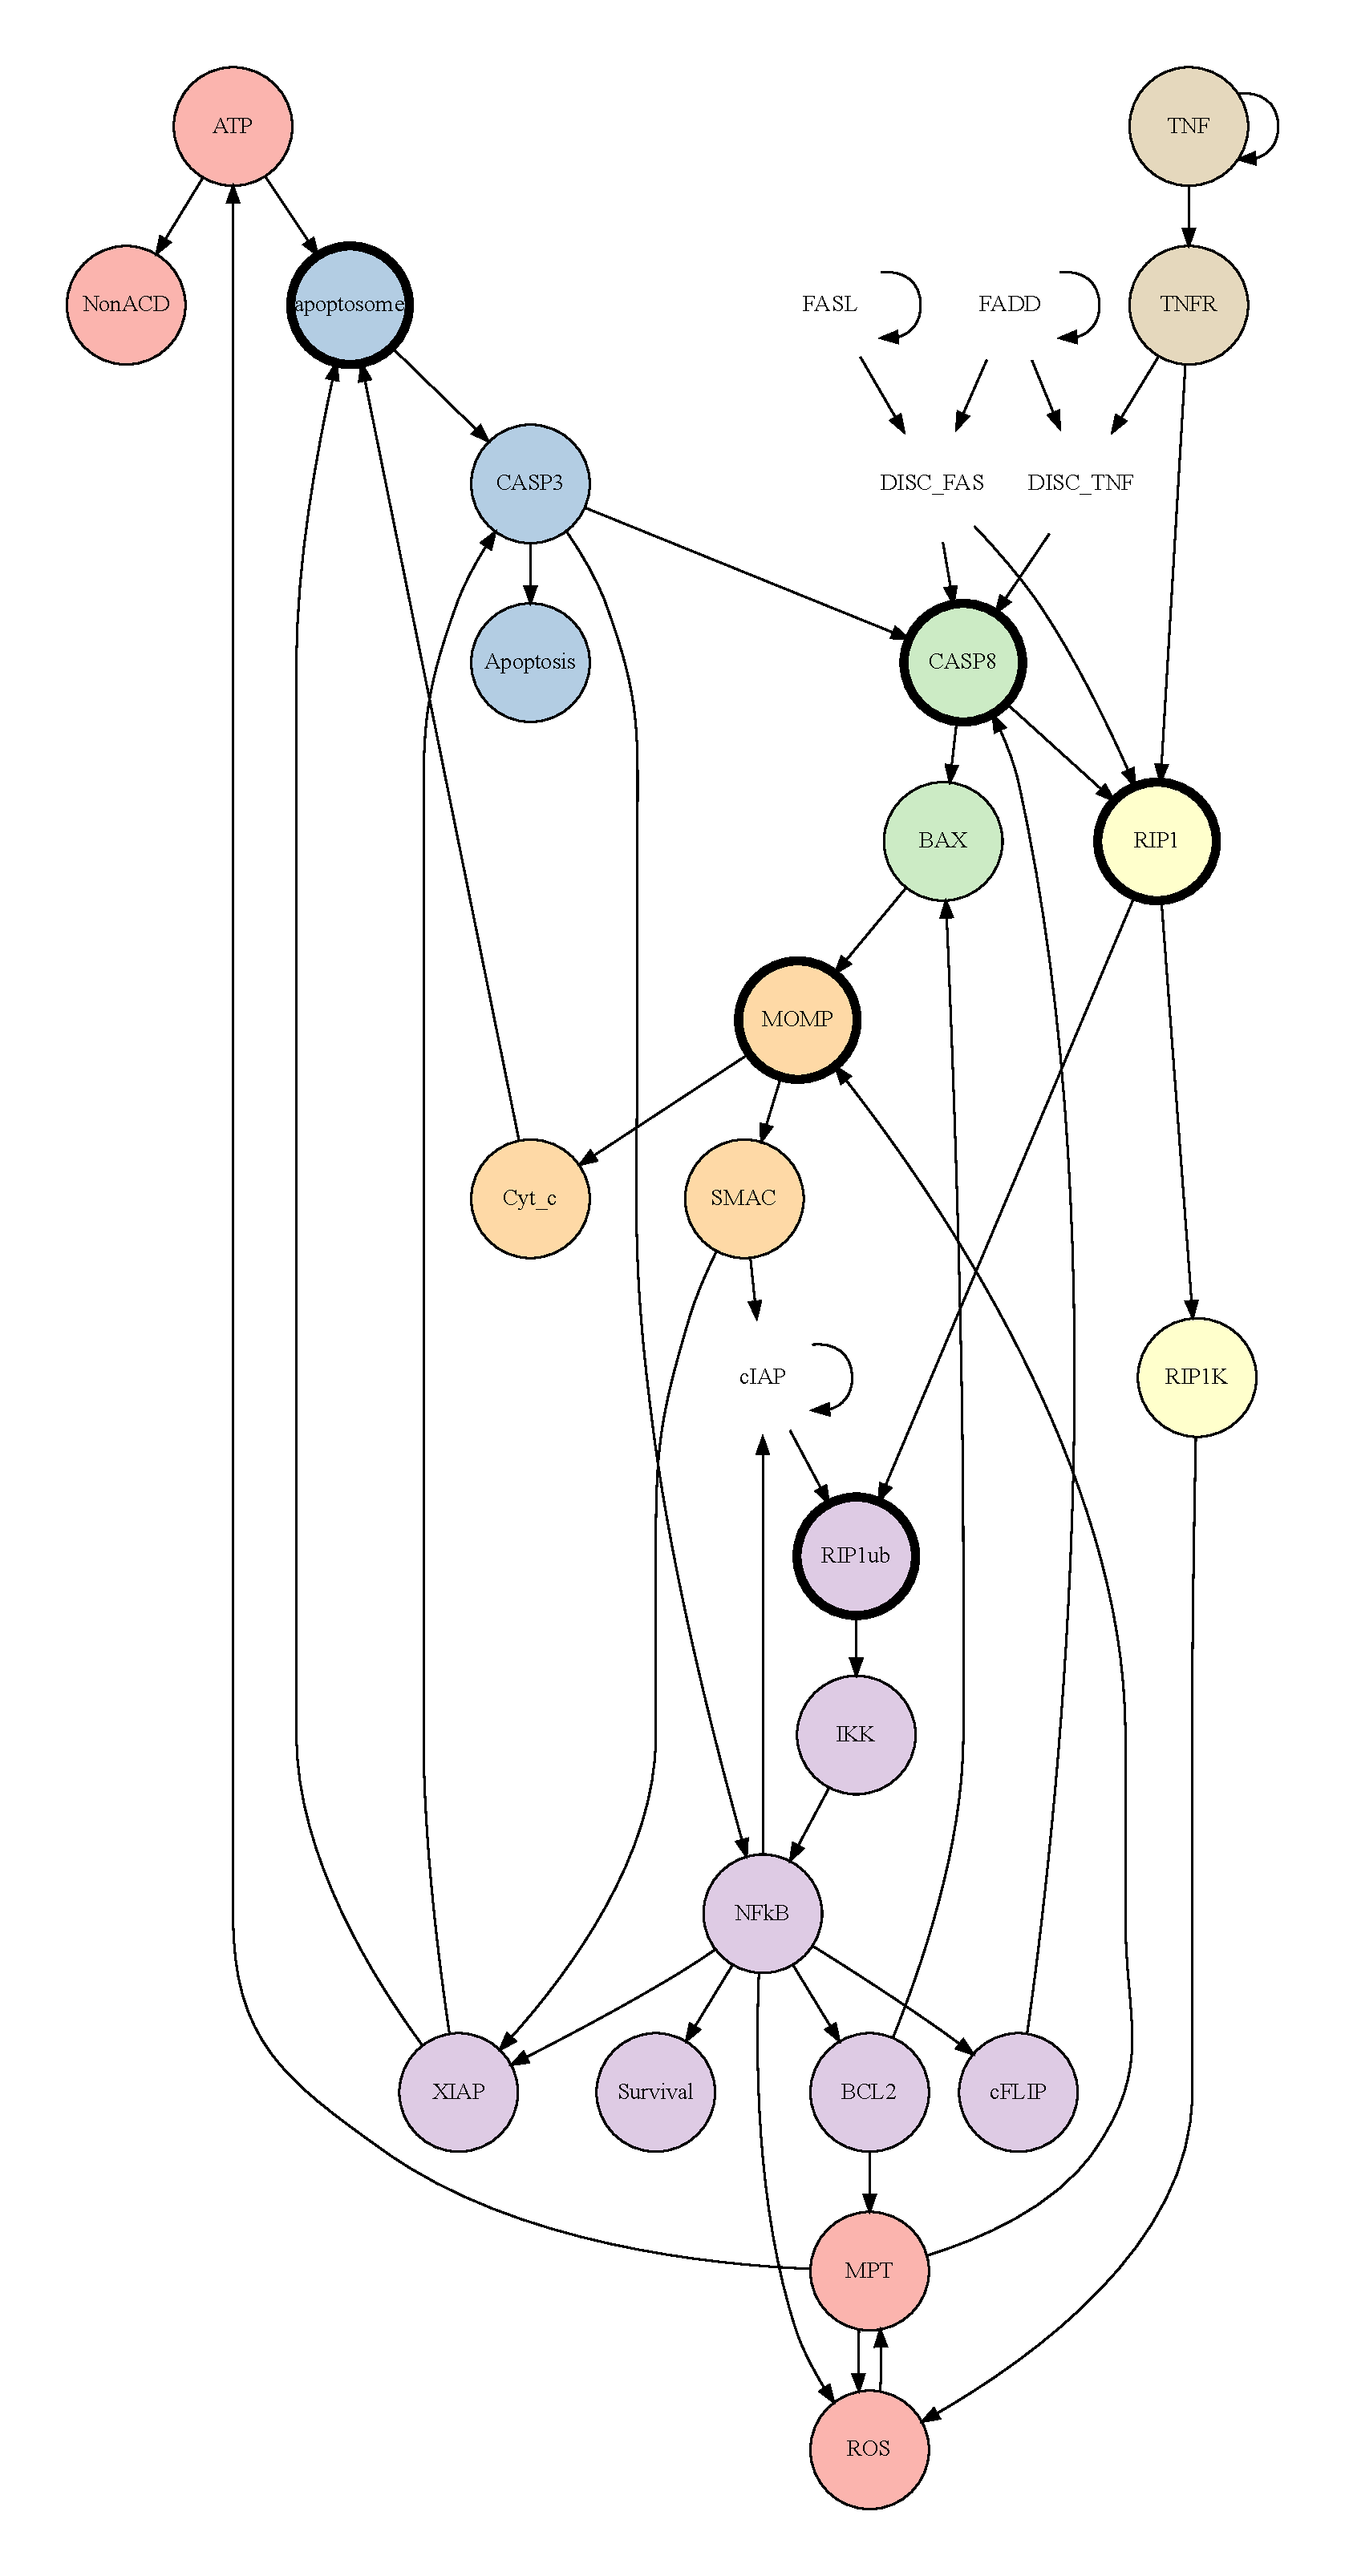
\includegraphics[width=0.7\linewidth]{igraph_steady_states}
        \caption{
            The blocks of the steady state correlation analysis of the death receptor model.
            Nodes without color belong to trivial blocks. Note that most blocks are tree-like.
            These have roots which can be seen as representatives of their blocks.
            They are highlighted with thick borders.}
        \label{fig:igraph-steady-states}
    \end{figure}

    We computed the subset minimal marker sets for four scenarios that are the result of all combinations of two binary parameters.
    The first parameter determines the consistency type between marker-type and phenotype.
    Its values are either \textit{1-to-1} or \textit{1-to-many}.
    The second determines whether the exclusion constraint for $P$ is enabled.
    Table~\ref{tab:calzone_markers} lists the marker families by number of components required and parameter values.
    The marker detection is solved instantly on a personal computer.

    \textbf{Scenario 1}: Subset minimality and equivalence required, exclusion constraint enabled.
    There are 126 markers, all of size 3.
    In set-product notation they are
    \[
        \{\{BCL2\},\{IKK\},\{NFkB\},\{RIP1ub\},\{XIAP\},\{cFLIP\}\} \otimes \mathbf L_1
    \]
    where $\mathbf L_1$ consists of 21 component pairs, including, for example $\{CASP3,MOMP\}$, $\{MPT,SMAC\}$, $\{MOMP,ROS\}$.
    An example of a valid marker set in this scenario is therefore $\{BCL2,CASP3,MOMP\}$.
    Note that the first factor corresponds to the purple block in the steady state correlation analysis of Figure~\ref{fig:igraph-steady-states}.


    \textbf{Scenario 2}: Subset minimality and consistency required, exclusion constraint enabled.
    In this scenario we require only consistency between marker-types and phenotypes, not equivalence.
    There are 324 markers of sizes 3, 4, 5, and we denote the respective subset of equal sized markers by $\mathbf X^3, \mathbf X^4, \mathbf X^5$.
    In set-product notation they are
    \begin{align*}
        \mathbf X^3 &= \{\{BCL2\},\{IKK\},\{NFkB\},\{RIP1\},\{RIP1K\},\{RIP1ub\},\{XIAP\},\{cFLIP\}\} \otimes \mathbf L_2\\
        \mathbf X^4 &= \{\{DISC\_FAS\}\} \otimes \{\{TNF\},\{TNFR\}\} \otimes \mathbf L_2\\
        \mathbf X^5 &= \{\{FADD\}\} \otimes \{\{FASL\}\} \otimes \{\{TNF\},\{TNFR\}\} \otimes \mathbf L_2\\
    \end{align*}
    where $\mathbf L_2$ consists of 27 pairs of components, including, for example $\{ATP,SMAC\}$, $\{CASP8,ROS\}$, $\{CASP3,Cyt\_c\}$.
    Note that the first factor of $\mathbf X^3$ is the union of the purple and yellow blocks in Figure~\ref{fig:igraph-steady-states}.
    Similarly, the factors of $\mathbf X^4, \mathbf X^5$ are unions of the trivial blocks \emph{FADD} and \emph{FASL} and the brown block.

    Examples of valid marker sets $\mathbf Y^3, \mathbf Y^4, \mathbf Y^5$ of sizes 3, 4 and 5 are therefore
    \begin{align*}
        \mathbf Y^3 &= \{RIP1, ATP, SMAC\}\\
        \mathbf Y^4 &= \{DISC\_FAS, TNF, CASP8,ROS\}\\
        \mathbf Y^5 &= \{FADD, FASL, TNF, CASP3,Cyt\_c\}\\
    \end{align*}

    \begin{table}
        \caption{The number of markers of the death receptor model for four different parameter combinations.}
        \label{tab:calzone_markers}
        \begin{minipage}{\columnwidth}
            \begin{center}
                \begin{tabular}{lllll}
                    \# marker components & \# marker sets & consistency type & exclusion constraint\\
                    \toprule
                    3& 126& 1-to-1 & active\\
                    \midrule
                    3& 231& 1-to-1 & inactive\\
                    \midrule
                    3& 216& 1-to-many & active\\
                    4& 54&  & \\
                    5& 54&  & \\
                    \midrule
                    3& 369& 1-to-many & inactive\\
                    4& 82&  & \\
                    5& 82&  & \\
                    \bottomrule
                \end{tabular}
            \end{center}
        \bigskip
        \end{minipage}
    \end{table}

    \section{Discussion}\label{sec:discussion}
    The results in this paper give theoretical foundations to a central problem in the design of multi-marker experiments.
    We have introduced a notion of consistency between markers and phenotypes and demonstrated that the enumeration of all subset minimal consistent marker sets is instantaneous for medium-sized Boolean networks.
    Furthermore, the steady state correlation analysis leads to an interesting tool, the map of interchangeable marker components of Fig.~\ref{fig:igraph-steady-states}.
    With it one may transform any valid marker set into other valid sets and detect, broadly speaking, clusters in the interaction graph that separate steady state information.
    It seems possible to extend the underlying relation $\sim_S$ from $V$ to $\mathcal P(V)$.
    This might be fruitful when further exploring the structure of marker families.

    The next steps are to validate the theoretical results of this work experimentally in a follow-up study on a recently published model of epithelial-to-mesenchymal transition (EMT), see~\cite{selvaggio2020hybrid}.
    Here, selected markers will be used to experimentally distinguish between cells that acquire distinct phenotypes on the EMT continuum during cancer progression.

    Also, the factorizations in Sec.~\ref{sec:results} are of a heuristic nature, and we do not yet have rigorous mathematical statements with regards to minimal factorizations.
    The product description seems promising, as it reveals 1) the number of independent choices and 2) the number of options for each choice.
    Research in this direction may lead to some notion of marker building blocks.

    \bibliographystyle{unsrt}
    \bibliography{markers_and_phenotypes}

\end{document}